%TODO: Intranet as not-proper name

%TODO: unique accesses per day
% todo set-up skills
% todo results of first questionnaire, also confirmed by future evolutions
% todo comparison with other organizations
% todo comparison with other committees
% todo importer, importance of professional kick-off
% todo importance of sandbox
% todo leadership
% todo initiation ritual (the makumba party)
% todo more precise hypotheses in intro
% todo direct access to other leaders  in method
% todo importance of mentoring for sust

%TODO refactoring as luxury, unlimited field of challenge diversification 
% TODO issue with questionnaire calendar years

% todo RUDI own data commentary for later integration
% todo RUDI initiation stories 

% DONE
% todo RUDI tables
%	=> just misses 2003, I'll see if i can get an estimate from Gwen tomorrow
% todo RUDI table/figure with quantitative questionnaire responses, per member, per skill
%	=> the one per member is not really readable... we could reduce it to show only people that stayed minimum 3 years, that's around 19 members. an image can be found in the repository, learning-members-2.png


% REMEMBER: After having produced the .bbl file,
% and prior to final submission,
% you need to 'insert'  your .bbl file into your source .tex file so as to provide
% ONE 'self-contained' source file.
%
% For tracking purposes - this is V3.0SP - JUNE 2007

\documentclass{acm_proc_article-sp}

\usepackage{url}
\usepackage{subfigure}

\begin{document}

\title{Makumba: the Role of the Technology for the Sustainability of Amateur Programming Practice and Community}
\subtitle{The Technological Religion of a Student Tribe}

% \numberofauthors{2}
% \author{
% \alignauthor
% Cristian Bogdan\\
%        \affaddr{School of Computer Science and Communication}\\
%        \affaddr{Royal Institute of Technology, 10044 Stockholm, Sweden}\\
%        \email{cristi@csc.kth.se}
% \alignauthor
% Rudolf Mayer\\
%        \affaddr{Institute of Software Technology and Interactive Systems}\\
%        \affaddr{Vienna University of Technology}\\
%        \affaddr{Favoritenstrasse 9--11, Vienna, Austria}\\
%        \email{mayer@ifs.tuwien.ac.at}
% }

% empty authors block for double-blind review
\numberofauthors{1}
\author{
\alignauthor
\hspace{10mm} \\
       \affaddr{\hspace{10mm} }\\
       \affaddr{\hspace{10mm} }\\
       \affaddr{\hspace{10mm} }\\
       \email{\hspace{10mm} }
}

\maketitle
\begin{abstract}
We address the issue of sustainability of practice, which we regard as crucial for the sustainability of the community at large. In the absence of material reward, sustaining a specialized activity such as programming is not a trivial matter especially when members move often in and out of the community. Our case is the group of voluntary, amateur student programmers from a European-wide student organization. We present this setting as an Amateur Community and as a Community of Practice, and show how such framing helps in understanding sustainability of practice. Although being totally voluntary and managing a large intranet, the group has been thriving for over ten years. To explain such high practice sustainability we examine the role of the technology framework used by the group, which was designed together with its members nine years ago. We then propose a more general framework for understanding practice sustainability in the context of amateur communities of practice. 
\end{abstract}

% see http://www.acm.org/about/class/ccs98-html
% however, http://cct2009.ist.psu.edu/papers.cfm does not seem to require them. and the topic is tough to fit.. we thus skip them

% A category with the (minimum) three required fields
%\category{H.4}{Information Systems Applications}{Miscellaneous}
%A category including the fourth, optional field follows...
%\category{D.2.8}{Software Engineering}{Metrics}[complexity measures, performance measures]

\keywords{Sustainability of Practice, Case studies, Amateur Community, Community of Practice} % NOT required for Proceedings

\section{Introduction}\label{sec:introduction}
The Intranet of an European-wide organization had just over 600 dynamic pages at its launch in 2002. The Intranet grew steadily in both size and functionality and at the end of 2008 it has almost 2000 dynamic pages. Throughout, except for a few glitches, the system was highly available and fast. Today the Intranet has around 2000 users from among the organization members, and its public part can be accessed by 4000-5000 organization customers at a time.

Such figures would not be surprising for a professional international organization, which hires or outsources professional programmers and system administrators. 
The figures are however unusual for a voluntary student organization, whose IT crew (referred to as the Tech Committee) is made of amateur voluntary student programmers who often do not study Computer Science or related subjects, or are at the early stages of their education.  
Since 2002, the Tech Committee had over 10 active members at any given time, and the Intranet was extended with more and more subsystems even if about one third of the Tech Committee membership was renewed each year. Reflection on this {\it sustainability} is the subject matter of this paper. We further assert that the design of the technology used to build the Intranet, called Makumba, is an essential ingredient of the Tech Committee sustainability.
Prior to Makumba introduction, the student organization had disparate IT systems, and the Tech Committee was formed in 1997 to maintain them but had much lower membership counts and was highly dependent on a few people.

In this paper we aim to characterize {\it sustainability of practice and community} based on this positive experience. We also aim to discuss the role of technology in achieving such sustainability, and to draw design implications that would help to devise technologies that encourage sustainability. 

While we recognize the importance of {\it environmental sustainability} in IT and interaction design \cite{blevis07}, we focus on a topic that is only abstractly related, yet we believe important in community and technology research. It is e.g. common knowledge that most virtual communities are "either young or dead" \cite{pargman05}, and various cookbooks for making the community thrive were produced \cite{goodwin94}. Even for non-virtual communities such as our student organization and its Tech Committee, it is sometimes difficult to sustain a specialized activity within the community, and this issue was raised under the name of sustainability in the field of Participatory Design (PD), e.g. as a basic principle of a PD method \cite{kensing98} or as a call for "self-sustaining [PD] processes within work settings" \cite{clement93}.  While managerial aspects such as leadership and incentives for work are certainly important in sustaining an activity, we also advocate a focus on the methods and tools used in such specialized activities, as them being easy to learn or entertaining to use should lead to better sustainability of the respective practice. As immediately apparent liabilities to practice sustainability one can exemplify lack of material rewards, or frequent changes in community membership, both of which affect voluntary student organizations. A related useful notion is {\it self-sustainability}, whereby a specialized activity such as PD \cite{clement93} or programming is started by professional intervention in the setting, yet it is able to continue using only community resources (human and otherwise), after the specialized professionals leave the setting. In our case both types of activity were initiated in the student organization  by the first author as a Human-Compute Interaction researcher and computer engineer, who left the setting in 2003. The programming activity and its sustainability are addressed in this paper.

In what follows, we will frame the Tech Committee as a Community of Practice \cite{lave_wenger91, wenger98} and as an Amateur Community \cite{bogdan03, bogdan_bowers07}. We will then introduce the topic of practice sustainability, highly related to learning and essential for community sustainability. We present the student organization's Intranet and the Makumba technology that powers it, then we describe in detail the sustainable evolution of the Intranet and the Tech Committee, as it comes out from examining the source code repositories and Tech Committee membership lists. We then present the results of several surveys 
%TODO: maybe just one survey?
that we used to elicit data on Makumba learning aspects in general and sustainability especially. We then discuss our results with a focus on learning, sustainability and design implications for technology.

%TODO maybe mention the dialog between authors if we manage to have it

\section{Setting}\label{sec:setting}
The student organization running the Intranet of our interest was grounded in 1988 and is currently present in 79 mainly technical universities across 30 European countries (grew from 60 in 2003), and currently has about 2500 members. Their aim is to organize {\it complementary education} in the form of courses and competitions for students of the member universities (i.e. not just for its members), to assist them with {\it career support}, and to foster the educational involvement of students through organizing symposia and workshops on different aspects of engineering education in Europe.
% TODO please add aims/details
The organization maintains contact with and raises funds from the European Union bodies and from a number of company partners. Internally, the organization has two statutory meetings per year and several less formal, smaller meetings in between. While most members only worked on international topics during such meetings, and for the rest they worked in their local organization chapters, since 1997 the organization was able to sustain "committees" on several topics: marketing, fund-raising, training and internal education, information technologies -- the Tech Committee, and complementary education program management. The committees met in the international meetings but kept on working on their topic also in between meetings, employing e-mail and instant messaging systems, as well as dedicated tools as part of the Intranet.

The Intranet is supporting the activities of the student organization. It was assembled as an integrated system in 2002 from several systems. The {\it first} such system was an event application system for complementary education courses. The system registered student applications to the course events, and let the organization manage their acceptance (to one event out of maximum three applied for) and participation. The system had been re-built yearly since around 1993 to different levels of completeness, including several years when it failed to work and the members had to resort to manual management. The application system was based on e-mail for communication initially, and a Web-based system was devised in 1995, built using the C programming language. The system finally 'stabilized' as a Java software which was re-used for several annual editions of the complementary education program starting in 1997. This system was helping the management of the most important student organization activity and was heavily dependent on the first author until its Makumba re-implementation completed in 2002.

The {\it second} system was an internal document archive and member profile management system known as the "Private Area". The system started as a set of manually maintained Web pages, keeping documents produced and voted upon in international meetings, and it was automated using Lotus Notes in 1998, when internal event management was added to facilitate member application to and participation in statutory meetings and other internal events. At the time, a need for a common technology for the IT systems of the organization was recognized and Lotus Notes was intended to be that technology. However its shortcomings for the Tech Committee context were recognized and the Makumba technology was designed in response.

{\it Third} a "virtual jobfair" was built as part of the 'career support' organization mission,  allowing companies to post job adverts, and students to post their profiles. This system was among the first coordinated implementation efforts of the Tech Committee, as different from the previous individual implementation endeavors. Several technologies were tried out, starting in 1997 with Lotus Notes, continuing with Java Servlet technology before the system was finally launched in 2000, using an incipient Makumba version.
% TODO, I think it was 2000, not sure how important this is, it was mostly unused for many years
% rudi: i think it was later, I'll try to dig it out

Besides heavily extending and integrating the above subsystems, several Intranet features were added since its inception: a Wiki, email archives for the organization's over 500 mailing lists, a training database, a survey-engine, a career-newletter, and a unique sign-in system that allowed students to share their accounts between the ``private area'', the course application system and the "virtual jobfair". Further, a number of support tools were implemented, like project and task management for both international committees and local chapters, company relations management for both the fund-raising committee and the local chapters, and several specific tools for the committees, often in the form of statistical analysis of number and increase of student accounts, subscription to the newsletters, etc. Another major new tool is an online voting system, intended to make the statutory meetings less crowded.
%TODO more here, it feels like little was done since 2002 :)
% rudi: still not enough? :-) i can still offer: teacher access to Johnny & possibility to share materials there,;IRC chat in PA; major improvements in document archives, events management; university project (university profiles & offers on the public site); PROP aka pr-ordering pages aka a web-shop for posters & materials; an FTP storage for LBGs, integrated in PA as applet & jsp pages viewing the data, based on PA accounts; several tools for LBGs to fetch data for their local webpages;

The Tech Committee is in charge of developing and maintaining the Intranet, as well as supporting it with activities such as helpdesk. The committee also coordinates activities of interaction design for further new areas of the Intranet. Administration of the Intranet, as well as of communication systems such as e-mail are also Tech Committee tasks. There are two formal membership levels ("trainee" and "active member") and there is a formal coordinator, elected each year, who is also a member of the student organization overall coordination bodies. In its early (less sustainable) days, the Tech Committee consisted of 1-5 members who were mainly responsible for the individual systems and had difficulties backing each other up when they did not have time for voluntary commitment. Membership levels increased after 2002, and new members are usually attracted in international meetings with a three-hour Makumba training, including exercises in making dynamic pages that browse Intranet data in various ways, improving existing Intranet pages, followed by assignment of more complex Intranet-related tasks.
% TODO more about the training, or after it: are they given Intranet tasks? Do they do Intranet-based exercises to change some interface or browse some Intranet data?
% rudi: in the training, they normally don't do intranet related tasks, they do completely new pages. they start from a given MDD, and then do the full range: list, object, newForm, and then for the more advanced ones also editForm, deleteLink, mak:count() & co.
% TODO rudi: not clear here, do you just want to describe the recruiting, or also the first path in ITC

\section{Methods}\label{sec:method}
We regard sustainability as a long-term matter that cannot be investigated with a short focused study. Throughout our contact with and involvement in the Tech Committee we were concerned with sustainability and at times we considered theoretical frameworks and recipes for how to achieve it, thus sustainability was an ever-present research issue for us, but also a practical issue in the community life. Both authors were active in the Tech Committee at different times (1997-2003 and 2004-2008 respectively), and {\it participant observation} was a conscious investigation approach for the first author, who also designed the Makumba technology together with Tech Committee members in a conscious act of {\it cooperative design} \cite{greenbaum_kyng91}. This paper is the occasion for a {\it reflection exercise} \cite{schon83}, on the part of the second author. Sustainability being a long-term issue, we expect other writings about it to be reflective accounts. 

We are highly aware that our first-hand involvement with the Tech Committee is a potential hinder for us producing an 'objective' account of its sustainability and on other matters of interest, and this is probably not uncommon in community-related research endeavors. We therefore complemented our personal experiences with both non-elicited and elicited data, as described below. Furthermore, our involvement having taken place {\it at different times} has resulted in a fruitful confrontation process that allowed us to depart from our personal opinions and arrive at more reliable and valid results.
%TODO more about dialog between authors
%TODO: rudi: here I'd add that we have seen a bit how it goes in other organizations, namely AEGEE, IAESTE, CFES, and to some extent bonding, though they have different settings with loads of meetings

For assessing quantitatively and qualitatively the sustainability of the Tech Committee and its practice, we regard as non-elicited data the {\it code repository} that the community has maintained, which allowed us to assess and reflect upon the progress of the Tech Committee work. The repository uses the Concurrent Versioning Systems (CVS) technology, which allows us to see the incremental changes and additions that were made to the code, their time, and their authors. We are thus able to reconstitute the Intranet code as it was at any moment in time since 2003. A number of code analysis tools are also available for investigating CVS repositories, and we found them useful for our inquiry.

We have also elicited data from the Tech Committee members, for purposes related to the Makumba technology. In 2002 the first author evaluated the design of Makumba with a questionnaire that had 12 respondents. In 2005 the first author also ran a questionnaire with 32 respondents to asses the status of Tech Committee work and technology use, and thus indirectly look at its sustainability. Finally, both authors designed a questionnaire at the end of 2008 where 30 out of the 45 past (since 2003) and present members who were approached reflected on their activity in the Tech Committee over their whole 3-4 year-long membership period. This questionnaire provides our paper with both quantitative and qualitative data. 
% parade 2005: http://private.best.eu.org/survey/admin/listAnswers.jsp?survey=fn29yq1
% makumba 2008: http://private.best.eu.org/survey/admin/listAnswers.jsp?survey=cwu9pab

During our membership we had access to the e-mail traffic and other communication of the Tech Committee. A further form of non-elicited data is constituted by Tech Committee {\it membership lists} at different times during the committee activity since 2002. Such lists can be made by examining member profiles in the Intranet. Number of members, as well as their level of activity are useful indicators in assessing sustainability. Therefore the membership lists were complemented with levels of member activity as elicited from committee leaders and self-assessed by members themselves in questionnaires. Personal acquaintance with many of the members and knowledge of their skill evolution has come to complement this further. Some members continued on an IT career after graduation, and this was yet another indicator of their Intranet development and generic IT skills. 

To be able to better comment on our data, we will go through some conceptualizations of learning, community, practice, amateur and voluntary work, and sustainability. We will also describe in more detail the design of Makumba.

\section{Community of Practice}\label{sec:cop}
Patterns of learning in the Tech Committee, as well as in the other committees and in the student organization at large, are well described by the Community of Practice social theory of learning  \cite{lave_wenger91, wenger98}. This learning perspective captures the social, informal and everyday aspects of learning, and emphasizes the community aspect of learning, i.e. members learn as part of and the ways of belonging to a community. This is referred to as "learning the ropes" or more formally "learning in doing".  As community members learn, they evolve from peripheral participants to 'full' community members, i.e. full participants. At first, they want, try, then pretend to be members, then they identify with the community and finally they become expert members. 
In effect this is a description of the social relations between newcomers and old timers, and of the individual acquiring of knowledge and skill. The process of becoming a full participant "configures" learning in doing.

This theory captures accurately the kinds of learning processes taking place in voluntary settings, where there is little incentive for attending elaborate formal education or resources for providing it. Instead, learning takes place while doing and participating, informally.
Practice is not all informal however, it is slowly reified \cite{wenger98} to canonical forms such as books of rules and regulations, training and other formal learning arrangements and material, etc. 

The Community of Practice perspective was extracted from field studies in five settings ranging from midwives to tailors and non-drinking alcoholics \cite{lave_wenger91}, but it of course applies well beyond, e.g. in insurance claim sorting \cite{wenger98}. Many programming-related activities and their 'learning/membership paths' covered by the community members are well-described by the theory, for example MUD community members becoming magicians (MUD programmers) \cite{pargman00, pargman05}, open source contributors becoming 'committers' i.e. earning the rights to commit new code to the open source project repository. It is worth noting that in both cases a formal, canonical member role has been reified out of existing practice, in a similar distinction to the trainee--full member reified in the Tech Committee.
% TODO: Rudi:  open source contributors ? i.e. you mean people that are already coding, but need to send their code to someone to check it? or you mean users of open source libraries, etc.. ?

\section{Amateur Community}\label{sec:amateur}
A further conceptualization that encompasses work in voluntary communities such as the Tech Committee, or other student groups, is the Amateur Community \cite{bogdan03, bogdan_bowers07}. The perspective was extracted from studies of Amateur Radio (ham) \cite{bogdan_bowers07} and has been tentatively applied also to open source and other programming related communities \cite{bogdan03}. 

The term 'amateur' is often used in a pejorative sense in everyday speech to denote 'novice', 'unprofessional', 'bad approach to work' or 'bad quality of work' . However, upon close examination of people who talk of themselves as being "amateur", authors have encountered that the skills of e.g. amateur mycologists \cite{fine98}, actors, baseball players and archaeologists \cite{stebbins79} range from novice-level to an expertise that rivals their professional counterparts. Sciences like astronomy still depend on the work of amateurs for their progress. Amateurs carry out their activities primarily out of their love (French "aimer") for the activities themselves, as different from paid (or otherwise rewarded) work activities such as jobs. An ethnographic account of various amateur settings \cite{stebbins79} describes amateurs as being socially situated "on the margin between work and leisure"; amateurs often describe their activity as work, and they rarely pursue it alone. Relevant social categories for amateurs are the \textit{professionals} of the activity that they pursue (e.g. professional radio operators for hams) which they draw influence from and sometimes exercise influence towards, and the \textit{public} towards which they relate in doing their work an benefit from it (e.g. the public at large in case of a disaster where amateur radio communication can be of help). This is referred to the Professional-Amateur-Public system. In relation to the professionals, amateurs can be professionals of their trade at the same time (e.g. hams who have jobs in the radio domain), or they may aspire to become professionals, in which case they are referred to as \textit{pre-professional}, or they have been professionals of the domain and presently continue it as amateurs (\textit{post-professionals}).

Within the Amateur Community perspective, amateur work is mainly driven by \textit{challenge}, which generally originates in \textit{contingencies} that need to be negotiated during the activity \cite{bogdan_bowers07}. Unlike professional work where contingency is often not welcome, and expensive to address (yet capacity to address it is regarded as competence), in amateur work contingencies of a specific kind are almost requisite. Amateur radio work is hampered by contingencies related to weather (which affects radio propagation), the working state of the radio equipment, what other hams happen to be active at the same time on the same frequency, how far they happen to be, etc. Yet it is these contingencies that constitute the radio challenge, addressed with pleasure by the members. The challenge, and its constitutive contingencies are thus requisite but must be \textit{addressable}, i.e. there should be enough skill within  the amateur community to address the challenge. At the individual level, balancing a challenge with skill is regarded as essential for the psychology of the optimal experience \cite{csik90}. A healthy \textit{contingency space} will include contingencies addressable by experts or old-timers as well as by novices or newcomers. For example, a novice ham operator can try to work short-range VHF connections (used routinely by the public for e.g. taxi cab dispatching)  while experts can try to achieve long-range VHF connections, preferably with low emission power, which have no public utility due to their lack of reliability, but constitute a great radio challenge.  

Besides being addressable with various levels of skill, a contingency space should ideally be \textit{inexhaustible}. In the amateur radio example, the weather is likely to always provide radio-related contingencies. On the contrary, an amateur community whose members aim to travel to all points of integer geographical latitude and longitude (www.confluence.org) have a remarkable, yet exhaustible contingency space. For a further example (also illustrating the diversity of amateur settings), amateurs who aim to teach re-populated bird species to migrate again by leading their flight with light aircraft (www.operationmigration.org) have a virtually inexhaustible contingency space, as increasing the number of re-populated birds, possibly in new places, is always valuable. Adding more bird species diversifies the challenge further. 

A further Amateur Community work driver is the \textit{audience} \cite{bogdan03}. Challenge addressing, shows of mastery are rarely kept for oneself. %TODO: doesn't sounds like a complete sentence..
Peers are normally expected to benefit from contingencies being negotiated, or members of the community \textit{public} will benefit. A notable form of community contribution is \textit{pioneering of new contingency spaces}.  For example ham operators who discovered new modes of radio propagation opened a whole new world for the rest of the amateur radio community, which other operators could chose to 'visit' or not, i.e. they could take the new challenge or just stay with the existing ones. Some such new forms of propagation were of direct benefit to the \textit{public}  (e.g. amplitude modulation) while others were only useful for the amateur community (e.g. connections achieved by sending a radio wave to the Moon which reflects it back to an Earth location where the other communication party is). Worth noting here is that challenge is \textit{socially constructed}, i.e. a new contingency space may be adopted by all or some community members, or it can be totally rejected as something that is not worth pursuing by the community.

\subsection{Amateur software development}\label{sec:amateur_devel}
It is useful to characterize amateur software development such as hackers \cite{levy94} or open source \cite{kollock99} as amateur communities 
because Tech Committee is a less professional (pre-professional) correspondent of such communities. 
Code challenge as hardly exhaustible, rich set of contingency, lots of trial and error, easy to open new contingency spaces also due to the immateriality of the working artifact. 
Challenge is addressable through high-skill of the members, yet sometimes module dependencies and opacity of architecture make novices have troubles. 
Audience and peer review are straightforward through e-mail and the code repository. Importance of plain text \cite{yamauchi00}. 
The community public is also straightforward and motivating (often world at large, or very skillful professionals).

\section{Sustainability of Practice in Amateur Communities}\label{sec:sust}
Now we have the concepts that are needed to better systematize sustainability in amateur communities.
Healthiness of  contingency space is actually sustainability. 
It means addressability of contingency at various levels of skill.
It also means inexhaustibility.
Sustainability can be both helped and hindered by challenge diversification.

Hypothesis: Need to have enough people at each difficulty level.

\section{Makumba, the Tech Committee tool}\label{sec:makumba}
Influences of Lotus Notes.
But plain text.
And few features.
Reduce complexities of professional technologies (e.g. types)
Levels of difficulty. How makumba is used. Smooth learning path (thesis page 166).
Populating a challenge (167).
The name... using a cultural term. Initiation rite. 
Introduction of Makumba, the importer done by the professional (first author) as it has no future/sustaining value anyway.

Inside the Tech Committee and the student organization, Makumba also plays an important role as a cultural element of the Tech Committee, namely in such a way that it is often associated with the \textit{Makumba party}, which happens during internal events of the organization, but is open only for Makumba users; TODO: group feeeling, etc.. 
Several mysteries entwine around those parties, which thus help to increase the curiosity of other members of the organization about Makumba and the Tech Committee, and can thus help in advertising tool for potential new members. TODO sounds a bit strangely formulated.

The Tech Committee also keeps a strong knowledge about it's own history and achievements, which are normally told to new members on the big annual summer meeting. Members feel proud to be part of a group that achieved pioneer things, like the first online application system in 1997 (TODO: ?), at a time when many companies had not even a static website, or inventing a technology similar to nowadays JSP, and most of all of Makumba, which was devised at a time when web-development frameworks were virtually non-existent.

\section{Sustainability of the Tech Committee}\label{sec:techCommittee}
\begin{itemize}
\item Tech Committee as an amateur community of practice
\item table with Karamba size, as it grew over years
\item table with number of members per year, at various makumba levels
\item some illustrative member trajectories (e.g. Gwen from little programming knowledge to Accenture, see chap 4 of thesis)
\item questionnaire commentary
\end{itemize}

\begin{table}
	\centering
	% TODO: explain LOC, etc? explain that all data is measured at the beginning of the year?
	% TODO: explain the drop from 2008 to 2009 needed? (due to removal of old BCC & public website pages in 2008, new ones have been added since late 2007, thus there were some ``duplicates'')
	\label{tab:intranet-size}
	\caption{Size of the Intranet}
	\begin{tabular}{c|r|r|r|r|r|r}
		\hline
		\hline
		Year	& MDD	& JSP	& BL	& \# files	& LOC		& CVS	 \\
		\hline
		\hline
		2002 	& 42	& 676	& 80	& 801		& 78479 	& N/A	 \\ 
		\hline
		2003 	& 52	& 961	& 116	& 1132		& 104805 	& 1143	 \\ 
		\hline
		2004 	& 64	& 1208	& 140	& 1415		& 127873 	& 702	 \\ 
		\hline
		2005 	& 76	& 1354	& 190	& 1628		& 151801 	& 1324	 \\ 
		\hline
		2006 	& 99	& 1719	& 229	& 2062		& 175315 	& 1632	 \\ 
		\hline
		2007 	& 111	& 2135	& 287	& 2559		& 219456 	& 2391	 \\ 
		\hline
		2008 	& 114	& 1860	& 289	& 2304		& 196867 	& 1898	 \\ 
		\hline
		
% old data, # files & LOC from CVS-stat
% 		Year		& \# files 		& LOC		& MDDs	& JSPs	& BL \\
% 		\hline
% 		\hline
% 		2003		& 850			& 55,000	& 42	& 729	& 80\\
% 		\hline
% 		2004		& 1,200			& 75,000	& 52	& 1097	& 116\\
% 		\hline
% 		2005		& 1,700			& 85,000	& 64	& 1388	& 140\\
% 		\hline
% 		2006		& 2,300			& 132,000	& 76	& 1564	& 190\\
% 		\hline
% 		2007		& 3,050			& 200,000	& 99	& 2057	& 229\\
% 		\hline
% 		2008		& 3,550			& 305,000	& 111	& 2526	& 287\\
% 		\hline
% 		2009		& 3,750			& 312,000	& 114	& 2303	& 289\\
		\hline
		\hline
	\end{tabular}
\end{table} 

Table~\ref{tab:intranet-size} shows the evolution of the size of The Intranet since it's launch seven years ago, detailed for the different technological levels MDD, JSP taglib and Business Logic. Additionally, the total number of code-related files is shown, along with the total lines of code (LOC). Besides those, several other files can be found in The Intranet application, such as javaScript libraries and self-developed scripts, a modified source-code branch of a Java/JSP Wiki-provider, and several layout files such as images and style-sheets; while those files surely add to the complexity of the application as a whole, managing them requires a different knowledge level than programming of database-driven web-applications -- they are thus omitted in our analysis.

Figure~\ref{fig:intranet-size} shows the evolution of the size graphically. It is worth noting that there was a rather high amount of MDD files defined in the beginning of The Intranet, representing data used in the first three sub-systems. Even though more data definitions have been added over time, a certain saturation level has been reached in the last years, with only minor additions. TODO: cristi says this is in-line with some data model stability, cite something?
In contrary, the amount of Business Logics files has continuously increased, with a leveling in the last year. This is because of the same reasons that lead to the decrease in JSP files in the last year -- in early 2008, the new version of the external parts of The Intranet (i.e. everything except the ``Private Area''), which features a totally new layout, and is integrated as one application. Development has however taken place mainly during 2007, keeping other development activities low, and for a certain time both the old and new version in the source code repository, until it was cleaned of the old JSP and Business Logics files in mid 2008.

\begin{figure}\label{fig:intranet-size}
  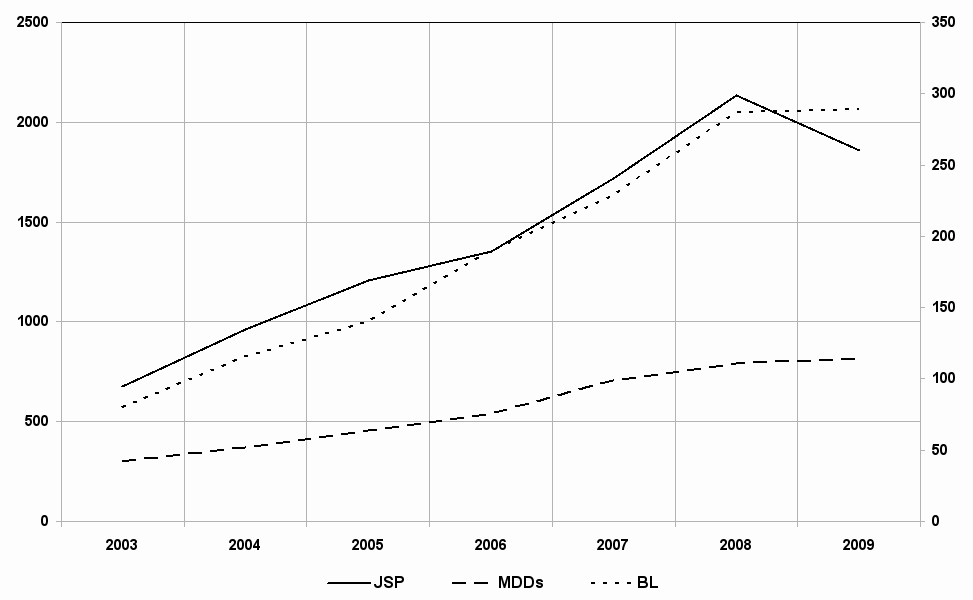
\includegraphics[width=0.98\columnwidth]{figures/SizeChart}
  \caption{Size of the Intranet}
\end{figure} 

Table~\ref{tab:intranet-size} illustrates the number of active members in the Tech Committee since 2004, differentiated on the different levels of Makumba, and on their activity in ``core'' and ``peripheral'' members. This data was on the one hand extracted from the questionnaire filled in by many of the members, and then refined and amended by some of the committee coordinators. Additionally, the number of members participating in the annual summer meetings, which are approximately one week meetings for all kinds of members, where besides designing features and planning the upcoming year also training and developing sessions take place, is depicted. It is interesting to note that while the overall number of active members increased over the years and stabilized in the last years, the number of members active on data definitions is not in-, but rather decreasing; this might be explained with the above described arrival at data maturity level, and thus less work and challenges to take for the Tech Committee members.

\begin{table}
	\centering
	\caption{Members in the Tech Committee}
	\label{tab:itd-members}
	\begin{tabular}{c|r|r|r|r|r|r|r|r|}
		\hline
		\hline
		Year 		& \multicolumn{2}{c|}{MDD} & \multicolumn{2}{c|}{JSP}	& \multicolumn{2}{c|}{BL}	& \multicolumn{2}{c|}{Total}	\\
					& Per & Core				& Per & Core				& Per & Core				& Per & Core	\\
		\hline
		\hline
		2003 & ? & ? & ? & ? & ? & ? & 4 & 5 \\
		\hline
		2004 & 3 & 4 & 7 & 3 & 3 & 3 & 6 & 5 \\
		\hline
		2005 & 5 & 6 & 8 & 11 & 7 & 3 & 8 & 13 \\
		\hline
		2006 & 7 & 8 & 9 & 12 & 9 & 3 & 10 & 12 \\
		\hline
		2007 & 7 & 7 & 14 & 9 & 10 & 5 & 12 & 11 \\
		\hline
		2008 & 6 & 5 & 13 & 7 & 6 & 7 & 12 & 8 \\
		\hline
		\hline
% Summer meetings
% 2003: http://private.best.eu.org/events/event.jsp?event=21-C-CJ-COM
% 2004: http://private.best.eu.org/events/event.jsp?event=22-C-RI-COM
% 2005: http://private.best.eu.org/events/event.jsp?event=23-C-LD-COM
% 2006: http://private.best.eu.org/events/event.jsp?event=24-C-SF-COM
% 2007: http://private.best.eu.org/events/event.jsp?event=25-C-TM-COM
% 2008: http://private.best.eu.org/events/event.jsp?event=26-C-BE-COM
	\end{tabular}
\end{table} 

\subsection{Survey}\label{sec:techCommittee-survey}
A survey was conducted among current and former members of the Tech Committee in the end of 2008, and filled in by 30 members. The background of the respondents is very diverse, ranging from their activity starting around 2001, to fresh members that just joined in the second half of 2008. Also the educational background is diverse -- seven members study computer science or engineering, while six study informatics; the other respondents study various different curricula, ranging from mechanical engineering over physics to biomedical engineering. Also, the membership duration in the committee varies, from half a dozen members that were active for around four years, to members that were (or currently are) active for one to two years. Most members had no knowledge of Makumba before joining, though some members, especially those active in other committees of the student organization (working closely with the Tech Committee) before joining, might have gotten some trainings (shortly) before.

The questionaire consisted of a total of 53 different questions, some were open questions, and others multiple-choice questions. The main focus was on gathering an understanding of the learning aspect of Makumba in the context of the Tech Committee, thus the participants were asked to answer several questions on their skill level on database design, SQL, general programming, Java, and three aspects of Makumba: JSP pages to view data, JSP pages to create, edit, and delete data, and business logics. The questions were for several different points in time, namely when joining the committee, and after the first, second, third and fourth year of membership, and allowed answers from ``no skills'' over ``little knowledge'', ``some experience'' and ``experienced'' to ``master''. To balance, and to facilitate, the different personal self-assessments, the participants were further asked to estimate their contribution to the committee in that year, and to list their projects and technologies the worked with in that year.

Figure~\ref{fig:learning-technologies} shows the averaged skill levels of all the members at different points in time. It can be observed that apparently, learning to view and display data is easier than handling forms to create, edit, and delete data, while Business Logics are the most difficult concept, especially in the first two years of membership. Most members that stay in the committee for a longer period, however, master all levels of Makumba almost equally well.

\begin{figure}\label{fig:learning-technologies}
  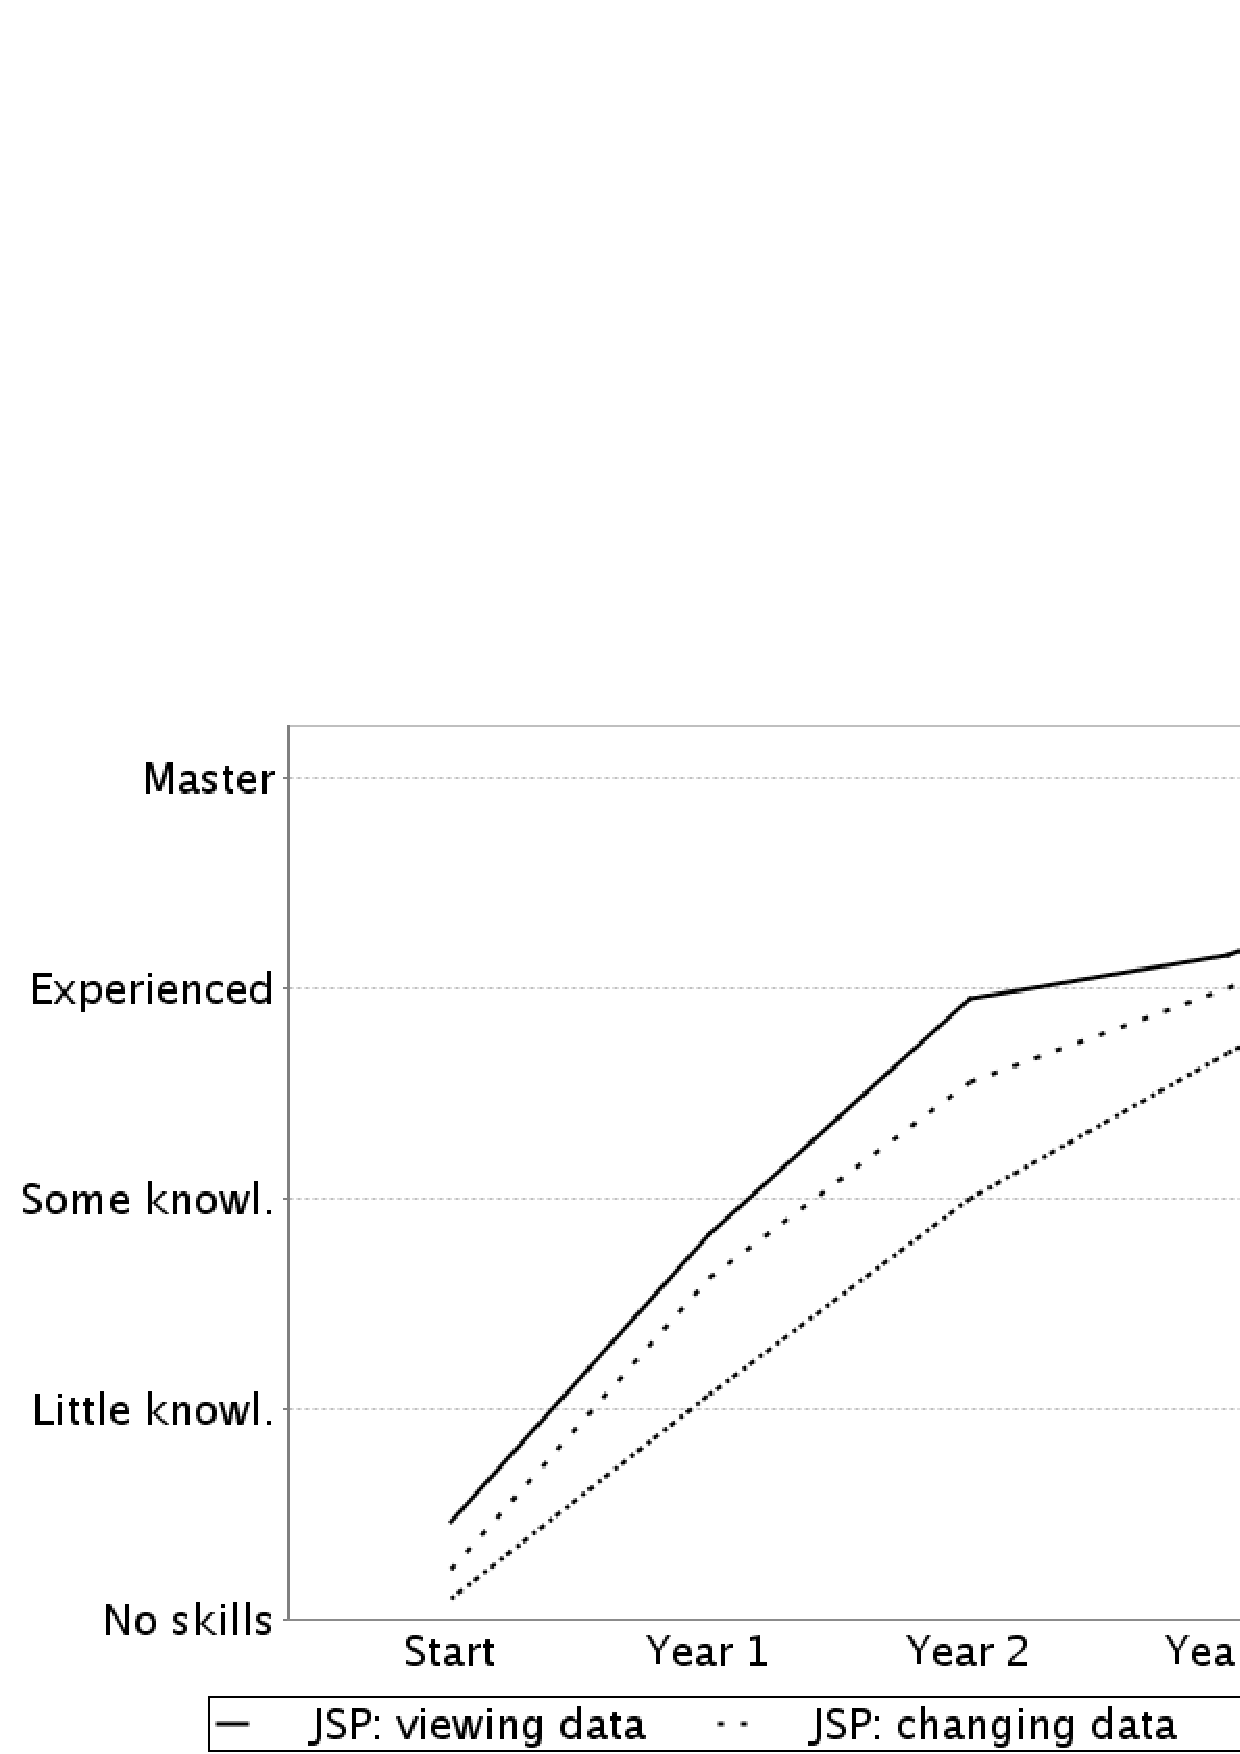
\includegraphics[width=0.98\columnwidth]{figures/learning-technologies}
  \caption{Learning curve for different aspects of Makumba}
\end{figure} 

Figure~\ref{fig:learning-members} shows skill trajectories for individual members, where the total skills on all Makumba technologies are simply summed up. From this graph, it can be observed that most members have a very steep skill rise in the first, and to some extent also in the second year. TODO: this is important due to high fluctuation... ?

% \begin{figure}\label{fig:learning-members}
%   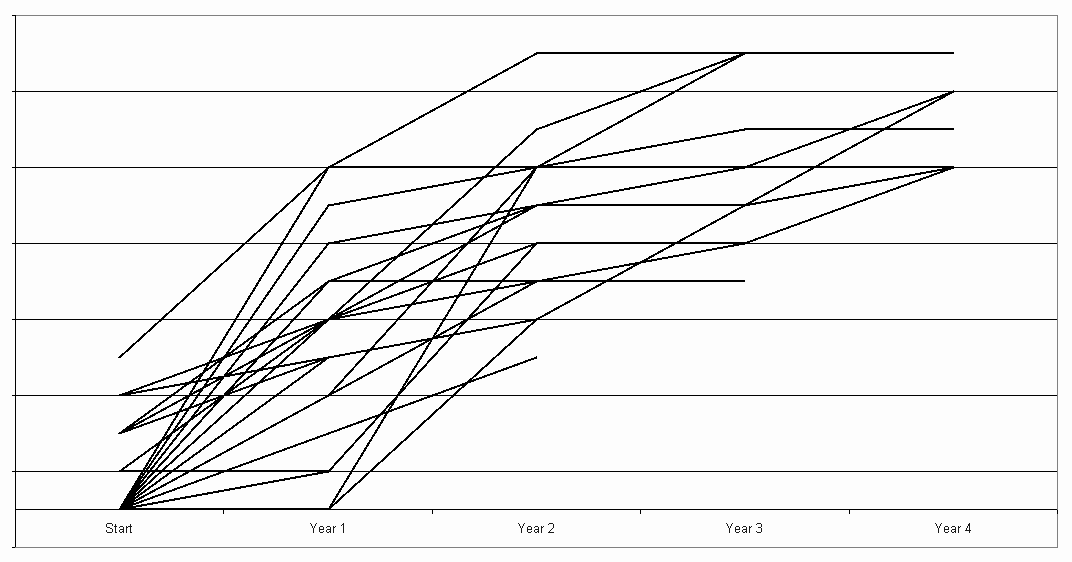
\includegraphics[width=0.98\columnwidth]{figures/learning-members}
%   \caption{Skill development of the survey respondents over the years}
% \end{figure} 

\begin{figure}
  \label{fig:learning-members}
  \caption{Skill development of selected survey respondents over the years}
  \subfigure[Julian]{
    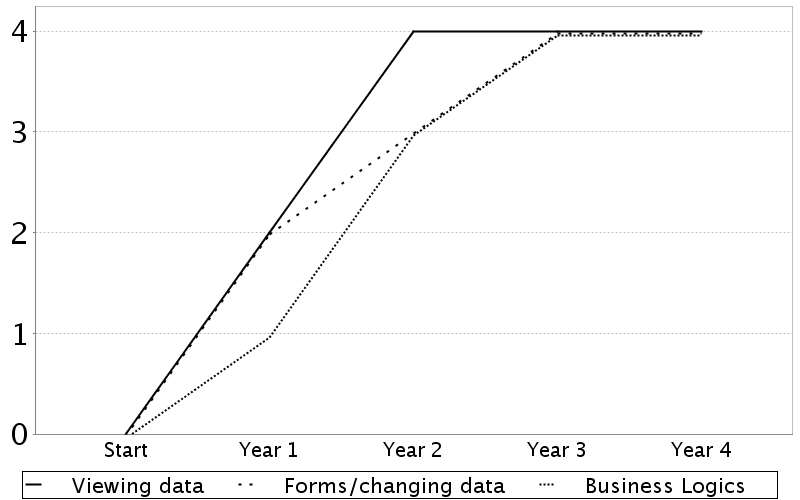
\includegraphics[width=0.22\textwidth]{figures/Joao}
    \label{fig:learning-members-joao}
  }
  \subfigure[Peter]{
    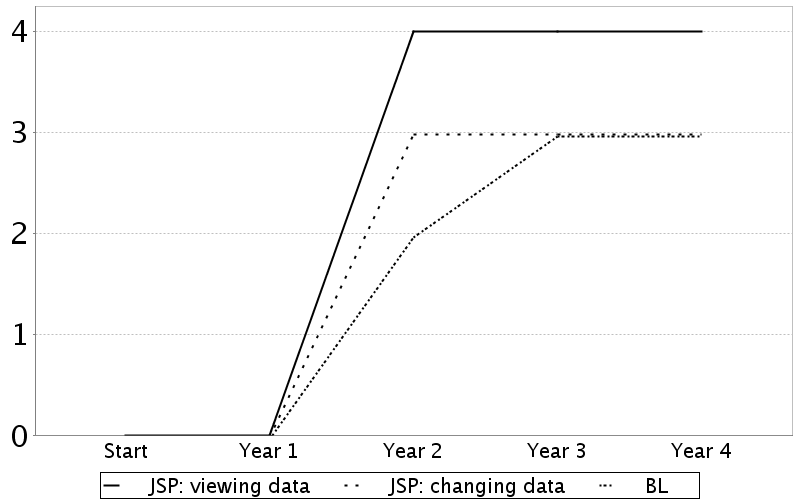
\includegraphics[width=0.22\textwidth]{figures/Priit}
    \label{fig:learning-members-priit}
  }
  \subfigure[Kim]{
    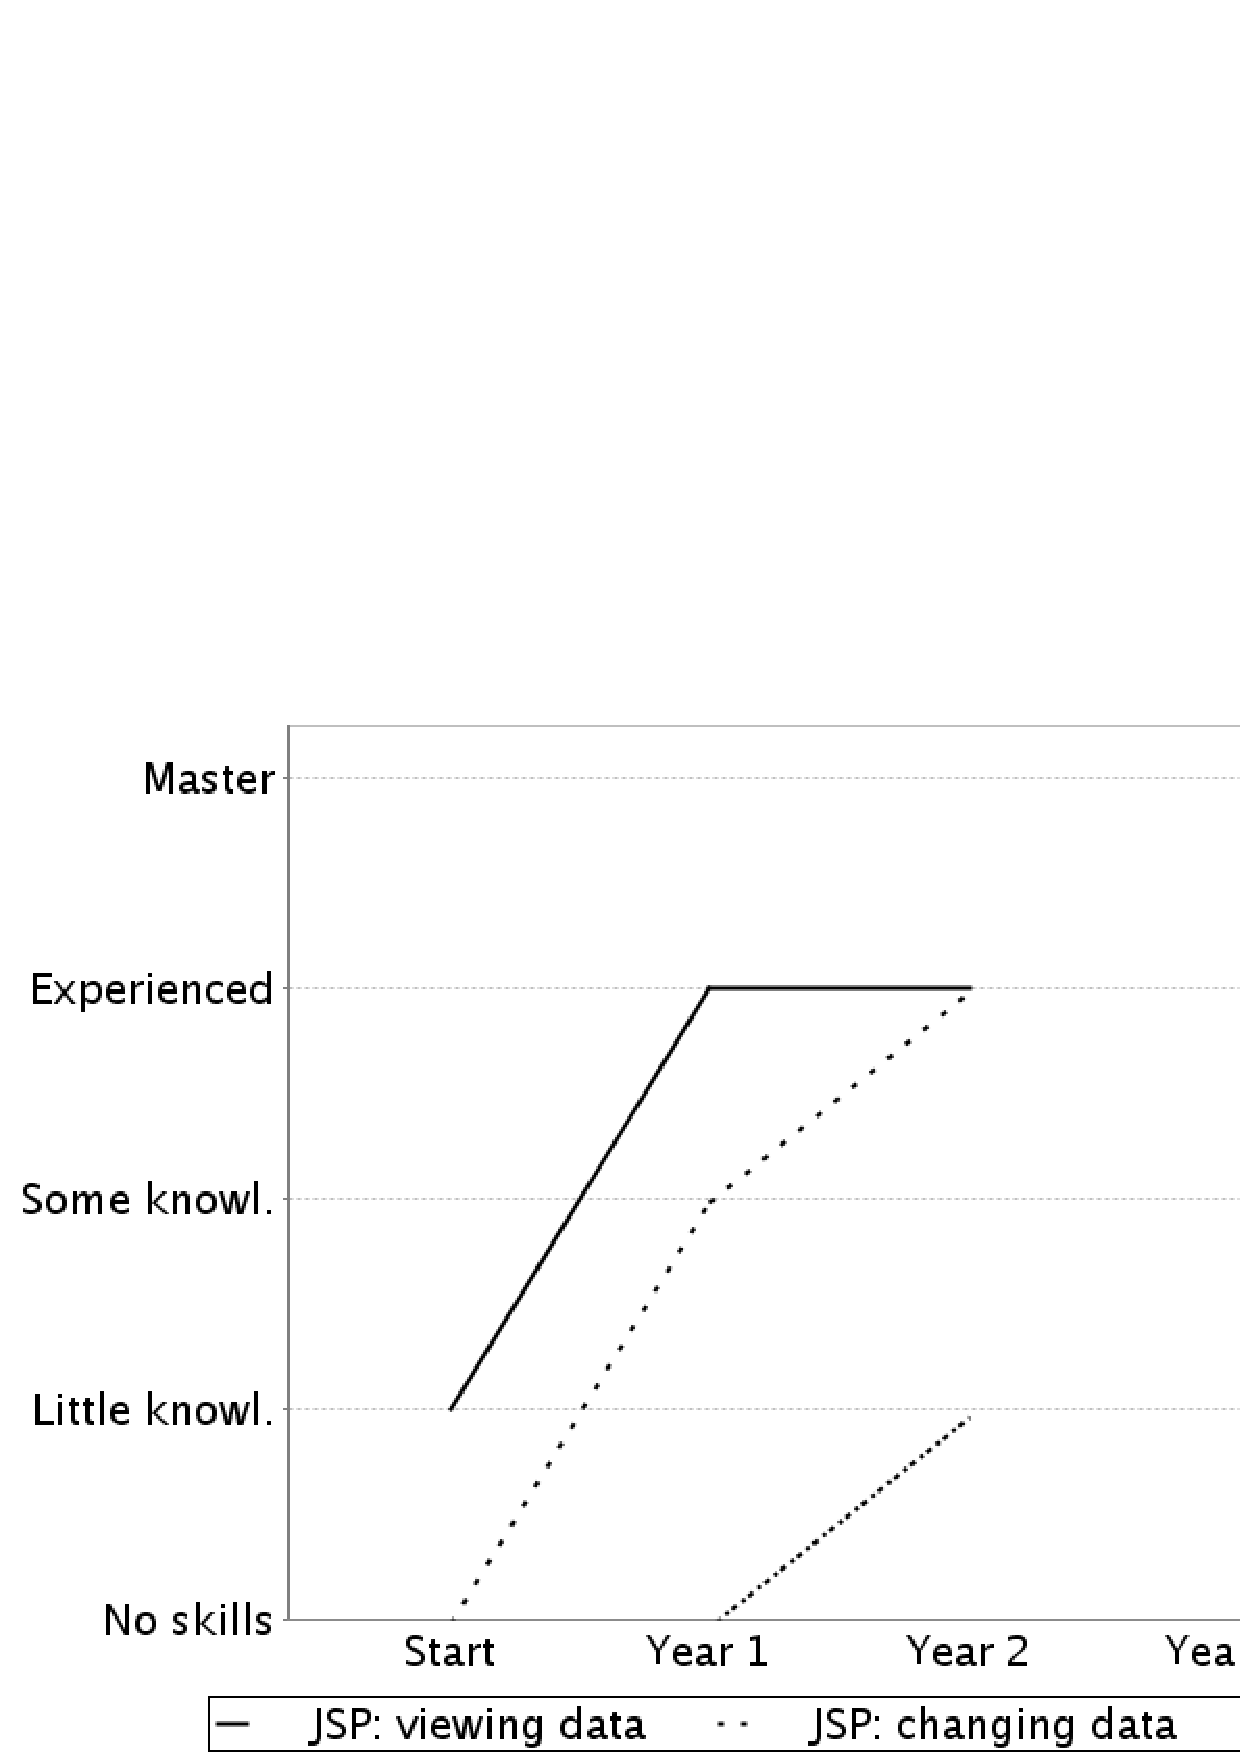
\includegraphics[width=0.22\textwidth]{figures/Karina}
    \label{fig:learning-members-karina}
  }
  \subfigure[Sam]{
    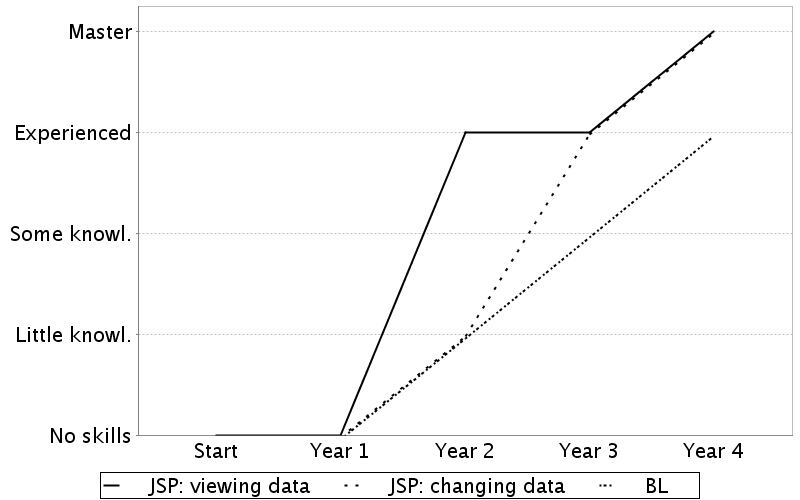
\includegraphics[width=0.22\textwidth]{figures/Stefan}
    \label{fig:learning-members-stefan}
  }
\end{figure} 




Finally, two open questions concluded the questionaire. The first one aimed at getting impressions on how the members experience learning technologies in the Tech Committee. Many people cited ``learning by doing'' and by using already existing pages as a base to be adapted to their needs as major factors; moreover, many developers stated how helpful the Tech Committee is with providing assistance with code examples, via the mailing list or chat channels. TODO: mention here that this alleviates lack of groups/forums/.. on the web?



% http://private.best.eu.org/survey/viewStatistics.jsp?survey=cwu9pab&graphs=true&comments=true
\begin{quotation}
 	% manu
 	"Learning by doing", "try and error" - the environment makes those two things possible, especially thanks to the ParaDe sandbox and the "linear" nature of Makumba/HTML. [..]\\
 	I would say that the code is very close to the result ("what you code is what you get"), or at least, very logically connected. 
\end{quotation}

\begin{quotation}
	The current systems provide a lot of examples - this has 2 sides: helps when you learn from the good examples, and makes it worse when you use the bad code. 
\end{quotation}

\begin{quotation}
	For me the greatest thing has been the first touch with coding using makumba: anybody is able to get a working page after 10 minutes of theory and 5 minutes of practice. That's provide motivation to do more difficult features.
\end{quotation}

\begin{quotation}
	I didn't attend any organised Makumba training, but learned the basics during events, in the first year. It was quite easy, although I didn't even know HTML or SQL when joining ITC. 
	(On the first 1-2 projects, I was directly helped by ITC experienced members). Afterwards, I started following also the emails and learned a lot from other people's problems/experiences.	
\end{quotation}

\begin{quotation}
	I usually learn by reading code and trying to reform it in a way that suits what i want to do. ITD is good at this part, since all our code is available and it's easy to find a place that something similar was done before. 
\end{quotation}

\begin{quotation}
	Learning is easy thanks to a lot of examples: for most of the tasks I could find another place where a similar feature had been implemented. Having a good knowledge about BEST IT systems helps more than having strong programming skills. Other ITD members also very often help and give advice when a problem or mistake occurs. 
\end{quotation}

\begin{quotation}
	Learning technologies in ITD is really easy cause we have a lot of documentation and a lot of people around in the ML eager to help. When I had a doubt, sending a mail to the list was enough to have 20 answers to the question explaining what to do, why and how :) 
\end{quotation}

\begin{quotation}
	Technology-wise, I love mak as how it's designed (the whole way the view/controller separation is less sharp than in other frameworks, how this is made very accessible and maintainable using the mak: tags, and how in the end this makes a large intranet maintainable by a community of people of variable skill), 
\end{quotation}

\begin{quotation}
	The ITD community is helpful, it is very easy to learn new technologies. I think makumba gives a very good starting point for learning web programming (separation of concerns, data model design). Everything that I learned in ITD has proved to be true also in the professional web development world. 
\end{quotation}

\begin{quotation}
	You get to learn new things both seeing what other do and by doing yourself. It is very easy to start doing things and see results very fast which is really motivating. 
\end{quotation}


The last question asked the respondents for a comparisons of Makumba with other technologies and frameworks aimed for web development.

\begin{quotation}
	All the other frameworks and technologies I know (Struts, PHP + templating engine, Zope) require a higher degree of computer technologies knowledge to achieve similar results. This might be changing with new frameworks like RoR in which the model definition is done in a similar way as in Makumba, but still I think RoR's learning curve is steeper than Makumba's 
\end{quotation}

\begin{quotation}
	I can only compare with PHP: PHP to start with was easy, but to make sound applications, you needed to do much more coding 
\end{quotation}

\begin{quotation}
	I did some basic JSP page with a blog in a school course I had, where we used HTML and JSP and mySQL for the database. This required many lines of code for doing the database connection and stuff. This was much easier in makumba, as you don't have to be get into all of this connection part and the database management in the same way. So having a solution like Makumba is much better for ITD where there is a bigger flow of students.
	(Of course it requires someone that also can take care of what's happening inside makumba, and this requires more knowledge and skills to do. So for a good suitability in ITD it's also important that there are people around that knows makumba from the inside.)
\end{quotation}

\begin{quotation}
	Makumba seems to work relatively fast "out-of-the-box" - Its very fast in Makumba to copy-paste and adapt "similar pages" to what you need. basically, you need to exchange the names of the MDDs used.. 
\end{quotation}

\begin{quotation}
	I have not used any other frameworks apart from writing my first PHP page this month (I wish I could have rewritten the whole app in makumba :)). Makumba still appears to me as having a very strong positioning, allowing to reach very quickly decent results with its basic features (allowing new joiners not to get tired of the learning effort and to contribute quickly) while also providing more powerful stuff for advanced users (allowing them to still find new challenges). 
\end{quotation}

\begin{quotation}
	Mak is significantly more suitable for ITD than anything else I've seen, despite the horrible inflexibility of the J2EE platform. Most other frameworks/setups insist on a very clear separation between the model and the view, and in most situations, this makes sense. However, by moving certain typically controller-world operations, such as database queries, to the view **in a simple and accessible way**, pages become much more maintainable without very strong documentation discipline, because they somewhat self-document.
\end{quotation}

\begin{quotation}
	Makumba being specifically designed for web applications, it is both extremely simple to learn for the basics - easier than PHP, especially for non-programmers - mainly through the easy interactions with databases ; yet can be as powerful as any other language, altough that involves dealing with Java, which is immediately more complicated - but not more complicated than any complex operation with any language.
	The main disadvantage is that everyone must learn it, since it is quite different from other web technologies. But the main advantage is that everyone \textit{can} learn, without too much of a technological background. I think that for ITC, or for any organization who wants to involve non-IT people in the development of their applications, the use of Makumba can make things much easier (provided that we keep having nerd masters to maintain and update it :p) 
\end{quotation}

\begin{quotation}
	Makumba is definitely the only technology suitable for BEST. I've been working a lot with trainees, teaching them the technology and about our systems, so after observing them it is quite clear that simplicity is the crucial aspect. Makumba is very easy to use and, with a bit of programming knowledge, BL is also quite accessible. One big advantage is the syntax, which makes it straight forward to understand other people's work. With Makumba, it doesn't happen so often that 2 people write totally different pieces of code for the same feature, and this is very useful for BEST (where people change very often). I would even say that, to some extent, Makumba is keeping me (and other people) in BEST. I would have never stayed so long in ITC, if it wasn't so easy and fun to learn Makumba. As well, the new features developed during the past year are so amazing, that it seems people are becoming active again just because they want to try them out! 
\end{quotation}

\begin{quotation}
	Makumba is really easy to use compared to other technologies. The learning time is short and the possibilities given by the framework are great. It's really fast to program with it and really user friendly. 
\end{quotation}

\begin{quotation}
	Makumba is great because it makes possible for non-IT people to write a webpage easily, with a little more knowledge than HTML
\end{quotation}

\begin{quotation}
	atm. I can't think of frameworks that do mix view and model, i.e. view and data query. they all go through a DAO layer, which would break the "what you code is what you get"). other frameworks also do have a lot of configuration overhead and rely on Java, which make it difficult for beginners to grasp. e.g. Struts needs to have several files changed in order to get a form to work, which is not so straightforward and slows down the "try and error" process. atm. I can't think of frameworks that do mix view and model, i.e. view and data query. they all go through a DAO layer, which would break the "what you code is what you get"). other frameworks also do have a lot of configuration overhead and rely on Java, which make it difficult for beginners to grasp. e.g. Struts needs to have several files changed in order to get a form to work, which is not so straightforward and slows down the "try and error" process. 
\end{quotation}

\subsection{Comparison with other student volunteer organizations}
The remarkable sustainability of the Tech Committee can also be illustrated by comparing the IT infrastructure with those of other similar student organizations the authors have had contact with; those contacts happened e.g. during the big statutory meetings of either the organizations, where a few delegates from the other organization were represented. In the last year, an increasing interest from other interests in the ``success story'' of the Tech Committee could be noted. Very close talks took place with AEGEE, which currently is in a similar situation as the Tech Committee was prior to introducing Makumba -- their systems are developed with different technologies, and their data is not connected. Currently, their major need is to have a working tool to keep track of membership in the local chapter -- which represents only a very small part of The Intranet of today;
TODO: AEGEE showed interest in copying a part of PA, the board of AEGEE even wanted to buy something..

CFES: have only very small document archive, called sharepoint. have no IT group, just a handful of members. periodically ask ITC for support, mainly on the general meetings.

IAESTE: no formal contact, just through some members. still do their job-exchange between local chapters by hand in their annual conference; application towards IAEST for  jobs with paper....


\section{Discussion}\label{sec:disco}
Our data show that designing a programming technology that allows member activity at various levels of skill, thereby prescribing a learning path for the members of the amateur community of practice, allows for sustainability of the amateur programming practice. In the case in point, we saw that the 'learning departments' of the setting, corresponding to the different programming languages used, were well populated at all times, in all our annual counts,  even if members left the setting every year. We can recommend as a design implication to design 'skill-modular' technologies, with 'modules' that require different levels of skill, with the first such module having a low learning threshold (HTML and SQL in the Makumba case) , in order to provide for addressability of challenge, and the next modules providing new challenge levels (e.g. BL in the Makumba case, with the procedural Java skill to be learned), thereby helping towards challenge inexhaustibility \cite{bogdan_bowers07}. Such learning modules with new challenges also provide for progressing from the periphery to the core, thus molding themselves well on Community of Practice social learning. The technology can then, as we believe Makumba does, be part of the configuration process emphasized by Lave and Wenger \cite{lave_wenger91}.

We were however not satisfied when discussing our data that this theoretical and mechanistic picture captures the Tech Committee sustainability entirely.The first author, who proposed it, has never actually worked in a sustainable Tech Committee, and has coded little of the the Makumba Intranet. It was the second author, along with former and present Tech Committee leaders during its sustainable days, who pointed out  several other aspects that lead to sustainability, some of which were confirmed by questionnaire respondents. First, the student organization regards Makumba as being something that \textit{belongs} to them. It is something that they give to the world therefore it is a way for them to relate to a \textit{public} \cite{stebbins79}, or a wide \textit{audience} \cite{bogdan03}, thereby increasing amateur motivation. Entering the Tech Committee gives one a privilege to work with a technology that is unique, and designed by previous Tech Committee generations. Entering the Tech Comittee also means being part of the team who had in 1995 an automated online application system at a time when many companies barely had a static website. While such an early achievement is not directly related to Makumba, it emphasizes the Tech Committee long-lasting tradition in the area of dynamic Web applications, Makumba's application domain, and is supplemented by other similar \textit{war stories} \cite{orr96} that have a role in learning, but also in creating a sense of belonging. Furthermore, entering the Tech Committee often means attending a Makumba party, one of these mysterious events that other people talked about but never wanted to give details. This reminds us of an \textit{initiation rite}\cite{vanGennep60} and plays a role in attracting new blood to the committee. In retrospect, choosing the Makumba name in favor of other, more technology-oriented but less student-community-oriented names was an inspired act. This teaches us that, while skill modularity has its merits, it can always use complementation from cultural meanings ascribed to the technology within the community: traditions, war stories, rituals, world-unique specificities. An implication then is to try to link the technology with community meaning. If this was possible to achieve (albeit somewhat accidentally) for such an intricate thing as a web development framework by a simple act of baptizing, it could work for many other technologies.

professional canons (m-v bl sep) and breaking them (non-dao)

scalability

all must learn, but that requires socialization

the luxury of refactoring, gardening

leadership

mentoring, adopted by other committees

sandbox, set-up skills

importer



\section{Conclusions}\label{sec:conclusions}

%ACKNOWLEDGMENTS are optional
\section{Acknowledgments}\label{sec:acknowledgments}
Thanks to the students, members and associates of the Tech Committee who have worked hard to overcome Makumba imperfections and to make the Intranet what it is today, while also taking time to answer our surveys.  Thanks are also due to all the non-BEST Makumba contributors.  Anonymous1 and Anonymous2 have supervised this work with good advice during the crucial Makumba design phases.

%
% The following two commands are all you need in the
% initial runs of your .tex file to
% produce the bibliography for the citations in your paper.
\bibliographystyle{abbrv}
\bibliography{cct2009-makumba} 

% For the final version:
% ACM needs 'a single self-contained file'!
%

\balancecolumns
% That's all folks!
\end{document}
